\documentclass[12pt, twoside]{article}
\usepackage{jmlda}
\newcommand{\hdir}{.}
\usepackage[utf8]{inputenc}
\usepackage[english,russian]{babel}
\usepackage{graphicx}
\newcommand{\real}{\mathbb{R}}
\newcommand{\nat}{\mathbb{N}}
\newcommand{\integ}{\mathbb{Z}}
\usepackage{bm}
\usepackage{multicol}
\usepackage{comment}


\begin{document}

\title
    [Анализ свойств ансамбля локально аппроксимирующих моделей] % краткое название; не нужно, если полное название влезает в~колонтитул
    {Анализ свойств ансамбля локально аппроксимирующих моделей}
\author
    [Р.\,И.~Исламов, А.\,В.~Грабовой, В.\,В.~Стрижов] % список авторов (не более трех) для колонтитула; не нужен, если основной список влезает в колонтитул
    {Р.\,И.~Исламов, А.\,В.~Грабовой, В.\,В.~Стрижов} % основной список авторов, выводимый в оглавление
    [Р.\,И.~Исламов$^1$, А.\,В.~Грабовой$^1$, В.\,В.~Стрижов$^{1}$] % список авторов, выводимый в заголовок; не нужен, если он не отличается от основного
\email
    {islamov.ri@phystech.edu; grabovoy.av@phystech.edu;  strijov@ccas.ru}
%\thanks
%    {Работа выполнена при
%     %частичной
%     финансовой поддержке РФФИ, проекты \No\ \No 00-00-00000 и 00-00-00001.}
\organization
    {$^1$Московский физико-технический институт}
\abstract
    {Данная работа посвящена построению универсальной модели в виде ансамбля локальных моделей. Для решения задачи регрессии  предлагается использовать ансамблевый подход. Множество объектов выборки разбивается на несколько подмножеств. Каждому подмножеству ставится в соответствие одна локальная модель, оптимально аппроксимирующая данное подмножество. Для аппроксимации выборки строится универсальный аппроксиматор. Он представлен в виде ансамбля локальных моделей. В качестве коэффициентов шлюзовой функции используется выпуклая комбинация локальных моделей. Ее значение зависит от объекта, для которого производится предсказание. Ансамблевый подход описывает те выборки, которые затруднительно описать одной моделью. Для анализа свойств ансамбля проводится вычислительный эксперимент. В качестве данных используются синтетические и реальные выборки. Исследуется расстояние между локальными моделями при оптимальном выборе параметров ансамбля. 
	
\bigskip
\noindent
\textbf{Ключевые слова}: \emph {восстановление регрессии; локальная модель; линейные модели; ансамбль моделей; универсальная модель.}
}

\maketitle
\linenumbers

\section{Введение}

Исследуются прикладные задачи, в которых данные порождены несколькими источниками. В таких случаях качество прогноза повышается с помощью использования нескольких моделей. Если моделей больше, чем нужно для получения требуемой аппроксимации, то веса избыточных моделей будут малы и их вклад в прогноз будет несущественен. Преимуществом ансамбля является его способность описывать те выборки, которые затруднительно описывать одной моделью.

В данной работе исследуется проблема построения ансамбля локальных моделей. \textit{Локальная модель} --- модель, которая аппроксимирует объекты, признаковые описания которых находятся в односвязной области пространства признаков. В качестве ансамблевой функции используется выпуклая комбинация локальных моделей. При этом веса локальных моделей зависят от положения объекта в пространстве признаков. 

В данной работе предполагается, что вклад каждой локальной модели в целевую переменную зависит от рассматриваемого объекта. Ансамбль локальных моделей использует шлюзовую функцию, которая определяет значимость предсказания каждой локальной модели, входящей в ансамбль. В данной работе каждая локальная модель является линейной. 

В качестве функции ошибки используется логарифм правдоподобия модели. Оптимальные параметры ансамбля и локальных моделей находятся при решении двухуровневой задачи оптимизации. На первом уровне оптимизируются параметры локальных моделей при фиксированных параметрах шлюзовой функции. На втором уровне оптимизируется параметры шлюзовой при найденных фиксированных параметрах локальных моделей. 

В данной работе исследуется расстояние между локальными моделями при различных параметрах шума. Расстоянием между локальными моделями является выборочный коэффициент корреляции Пирсона. Предполагается, что локальные модели тем дальше находятся друг от друга в пространстве локальных моделей, чем ближе коэффициент корреляции к нулю.

Оптимальный алгоритм тестировался на синтетических и реальных данных.  Эксперименты показали преимущество использования ансамбля локальных моделей по сравнению с использованием одной модели. Эксперимент также показал, что при увеличении параметра шума локальные модели отдаляются друг от друга, становятся независимыми.

Ансамблевый подход стал предметом многих исследований. Ансамбль моделей использовался в работах~\cite{Yumlu2003, Cheung1995, Weigend2000}. В работе~\cite{Yuksel2012} представлен обзор методов и моделей в задачах ансамбля моделей. В данной работе представлены виды шлюзовых функций. Приведен анализ разных моделей, которые могут выступать в качестве локальной модели. 

Ансамблевый подход имеет множество приложений в прикладных задачах. В работе~\cite{article} предложен метод распознавания рукописных цифр. Метод распознания текстов при помощи ансамбля локальных моделей исследуется в работах~\cite{Estabrooks2001}, а для распознавания речи~---~в~\cite{Mossavat2010, Peng1996}. В работе~\cite{Sminchisescu2007} исследуется ансамбль локальных моделей для задачи распознавания трехмерных движений человека.


Были предложены различные типы локальных моделей, такие как SVM~\cite{Collobert2002}, Гауссовский процесс~\cite{Tresp01mixturesof}  и нейронные сети~\cite{Shazeer2017}. Другие работы была сосредоточены на различных конфигурациях, таких как иерархическая структура~\cite{NIPS1991_514}, бесконечное число экспертов~\cite{Rasmussen} и последовательное добавление локальных моделей~\cite{Aljundi2016}. Работа~\cite{garmash-monz-2016-ensemble} предлагает модель ансамбля локальных моделей для машинного перевода.  



\section{Постановка задачи построения ансамбля локальных моделей}

Задано множество объектов $\Omega$, признаки которых описываются матрицей
\[\mathbf{X} \in \real^{N\times n}, \eqno(2.1)\]
где~$N$~---~число объектов во множестве, а~$n$~---~размерность признакового пространства. Каждому объекту~$\omega_i$ из~$\Omega$ соответствует признаковое описание~$\mathbf{x}_i \in \real^n$, которое является~$i$-ой строкой матрицы~$\mathbf{X}$, и значение целевой переменной~$y_i \in \real$.  Введем выборку данных~$\mathfrak{D}$:
\[\mathfrak{D} = \{(\mathbf{x}_i, \mathrm{y}_i)~|~ i \in \overline{1, N}\}. \eqno(2.2)\]

В данной работе предполагается, что выборка~$\mathfrak{D}$ порождена~$K$ источниками. Это предположение индуцирует разбиение множества индексов~$\mathcal{I} = \{1, 2, \dotsc, N\}$ на~$K$ непересекающихся подмножеств~$\mathcal{I}_k$:

\[\mathcal{I} = \bigsqcup\limits_{k=1}^K \mathcal{I}_k. \eqno(2.3)\]
Разбиение индексного множества~$\mathcal{I}$ индуцирует разбиение множества объектов~$\Omega$ на подмножества~$\Omega_k$

\[\Omega = \bigsqcup\limits_{k=1}^K \Omega_k, \qquad \Omega_k = \{\omega_i \in \Omega~|~i \in \mathcal{I}_k\}\eqno(2.4)\]
и выборку $\mathfrak{D}$ на подвыборки $\mathfrak{D}_k$

\[\mathfrak{D} = \bigcup\limits_{k=1}^K \mathfrak{D}_k, \qquad \mathfrak{D}_k = \{(\mathbf{x}_i, \mathrm{y}_i) \in \mathfrak{D}~|~i \in \mathcal{I}_k\}.\eqno(2.5)\]
Для каждого подмножества объектов~$\Omega_k$ используется своя локальная модель.\\
\begin{Definition}
\label{def:1}
Модель~$\mathrm{g}_k$ называется локальной, если она аппроксимирует аппроксимирует подвыборку $\mathfrak{D}_k = \{(\mathbf{x}_i, y_i) \in \mathfrak{D}~|~i \in \mathcal{I}_k\}$.
\end{Definition}
В данной работе локальный модели объединены в ансамбль локальных моделей.\\
\begin{Definition}
\label{def:2}
Ансамбль локальных моделей --- мультимодель, определяющая правдоподобие веса~$\pi_k$ каждой локальной модели~$g_k$ на признаковом описании объекта $\textbf{x}$.
\[\mathrm{f} = \sum\limits_{k=1}^K\pi_k \mathrm{g}_k(\mathbf{x},\mathbf{w}_k),\qquad \pi_k\left(\mathbf{x}, \mathbf{V}\right): \real^{n\times |\mathbf{V}|} \rightarrow [0,1], \qquad \sum\limits_{k=1}^K\pi_k\left(\mathbf{x}, \mathbf{V}\right) = 1, \eqno(2.6)\]
где~$\mathrm{f}$~---~ансамбль локальных моделей, $\mathrm{g}_k$~---~локальная модель, $\pi_k$~---~шлюзовая функция, $\mathbf{V}$~---~параметры шлюзовой функции. 
\end{Definition}



В работе в качестве локальной модели $\mathrm{g}_k$ используется линейная модель, а в качестве шлюзовой функции $\bm{\pi}$ используется двухслойная нейросеть:

\[\mathrm{g}_k(\mathbf{x}, \mathbf{w}_k) = \mathbf{w}_k^{\mathsf{T}}\mathbf{x}, \qquad \bm{\pi}\left(\mathbf{x}, \mathbf{V}\right) = \text{softmax}\bigg(\mathbf{V}_1^{\mathsf{T}}\bm\sigma\left(\mathbf{V}_2^{\mathsf{T}}\mathbf{x}\right)\bigg), \eqno(2.7)\]
где~$\mathbf{V} = \{\mathbf{V}_1, \mathbf{V}_2\}$~---~параметры шлюзовой функции, $\sigma(x)$~---~сигмоидная функция. Вводится понятие расстояние между двумя объектами.\\
\begin{Definition}
\label{def:3}
Расстоянием между двумя объектами~$\omega_1$ и~$\omega_2$ из~$\Omega$ называется число, равное расстоянию между векторами~$\mathbf{x}_1, \mathbf{x}_2$ признаковых описаний этих объектов:

\[\rho(\omega_1, \omega_2) = ||\mathbf{x}_1 - \mathbf{x}_2||_2. \eqno(2.8) \] 
\end{Definition} 

В пространстве локальных моделей вводится расстояние между локальными моделями, равное выборочному коэффициенту корреляции Пирсона.\\
\begin{Definition}
\label{def:4}
Расстояние между двумя локальными моделями $\mathrm{g}_i$ и $\mathrm{g}_j$ на выборке $\mathbf{X}\in\real^{N\times n}$ вычисляется по формуле
\[\rho(\mathrm{g}_i, \mathrm{g}_j) = \frac{\sum\limits_{l=1}^N \left(\mathrm{X}_{il} - \overline{\mathrm{X}}_{i}\right)\left(\mathrm{X}_{jl} - \overline{\mathrm{X}}_{j}\right)}{\sqrt{\sum\limits_{l=1}^N \left(\mathrm{X}_{jl} - \overline{\mathrm{X}}_{j}\right)^2 \sum\limits_{l=1}^N \left(\mathrm{X}_{jl} - \overline{\mathrm{X}}_{j}\right)^2}}, \eqno(2.9)\]
где $\mathrm{X}_{il} = (\mathbf{X}\mathbf{w}_i)_l, \mathrm{X}_{jl} = (\mathbf{X}\mathbf{w}_j)_l, \overline{\mathrm{X}}_i = \frac{1}{N}\sum\limits_{l=1}^N \mathrm{X}_{il}, \overline{\mathrm{X}}_i = \frac{1}{N}\sum\limits_{l=1}^N \mathrm{X}_{il}, \mathbf{w}_i$~---~параметры локальной модели~$\mathrm{g}_i$, $\mathbf{w}_j$~---~параметры локальной модели~$\mathrm{g}_j$.
%%%\mathsf{cov}\bigg(\mathbf{g}_i(\mathbf{x},\mathbf{w}_i),\mathbf{g}_j(\mathbf{x}, \mathbf{w}_j) \bigg) = \mathsf{E}\bigg(\stackrel{\mathsf{o}}{\mathbf{g}}_i(\mathbf{x}\cdot \mathbf{w}_i)\cdot\stackrel{\mathsf{o}}{\mathbf{g}}_j(\mathbf{x}, \mathbf{w}_j) \bigg), \eqno(2.9)\]
\end{Definition}
Данное определение можно интерпретировать следующим образом: чем ближе расстояние между моделями к нулю, тем дальше находятся локальные модели друг от друга в пространстве моделей, и наоборот.


Для нахождения оптимальных параметров мультимодели используется функция ошибки следующего вида:
\[\mathcal{L}\left(\textbf{V}, \textbf{W}\right) = \sum\limits_{(\textbf{x}, y) \in \mathcal{D}} \sum\limits_{k=1}^K\pi_k\left(\textbf{x}, \textbf{V}\right)\left(y - \textbf{w}_k^{\mathsf{T}}\textbf{x}\right)^2 + R\left(\mathbf{V}, \mathbf{W}\right), \eqno(2.10)\] 
где $\mathbf{W} = [\mathbf{w}_1, \mathbf{w}_2, \dotsc, \mathbf{w}_k]$ --- параметры локальных моделей, $R\left(\mathbf{V}, \mathbf{W}\right)$ --- регуляризация параметров. Оптимальные параметры определяются из выражения

\[\hat{\mathbf{V}}, \hat{\mathbf{W}} = \argmin\limits_{\mathbf{V}, \mathbf{W}}{\mathcal{L}\left(\textbf{V}, \textbf{W}\right)}. \eqno(2.11)\]

В качестве базового алгоритма используется ЕМ-алгоритм. Алгоритм подробно описан в \cite{Bishop2011}. Формулы, по которым происходит оптимизация функции ошибки $(2.11)$, приведены в работе \cite{Grabovoy2020}. 

\section{Вычислительный эксперимент}

\subsection{Цель эксперимента}

Данный эксперимент ставится для того, чтобы показать, что одна линейная модель плохо аппроксимирует выборку, объекты которой порождены несколькими источниками.

В качестве данных используются синтетическая выборка. Рассмотрим две подвыборки объектов, имеющих по одному признаку $x_m$, описываемых линейной моделью с нормальным шумом:
\[\mathrm{y}_m = \alpha_{m}\mathrm{x}_m+ \varepsilon,   \qquad \mathrm{x}_m, \mathrm{y}_m \in \real, \qquad m \in \{1,2\}, \qquad \varepsilon \in \mathcal{N}(0, 1). \eqno(3.1)\] 
В качестве общей выборки рассматривается конкатенация двух подвыборок, описываемая вектором целевой переменной $\mathbf{y}$ и матрицей признаков $\mathbf{X}$:	
\[\mathbf{y} = \begin{pmatrix}
\mathrm{y}_1\\
\mathrm{y}_2
\end{pmatrix}, \qquad\mathbf{X} = \begin{pmatrix}
\mathrm{x}_1 & 0\\
0 & \mathrm{x}_2
\end{pmatrix}.\eqno(3.2)\]

На общей выборке $\mathbf{X}$ обучается линейная модель. Линейная модель хорошо аппроксимирует данную выборку (см. рис. $1\text{a}$). 

Во втором эксперименте две подвыборки сливаются в одну общую выборку, описываемая целевой переменной $\mathbf{y}$ и матрицей признаков $\hat{\mathbf{X}}$:
\[\mathbf{y} = \begin{pmatrix}
\mathbf{y}_1\\
\mathbf{y}_2
\end{pmatrix}, \qquad \mathbf{\hat{X}} = \begin{pmatrix}
\mathrm{x}_1 & \varepsilon_1\\
\varepsilon_2 & \mathrm{x}_2
\end{pmatrix},\eqno(3.3)\]
где $\varepsilon_1, \varepsilon_2 \in \mathcal{N}(0,1)$. На построенной модели также обучается линейная модель. В этом случае линейная модель плохо аппроксимирует данную выборку (см. рис. $1\text{б}$). 




\begin{figure}[h]
\begin{center}
\begin{minipage}[h]{0.49\linewidth}
\begin{center}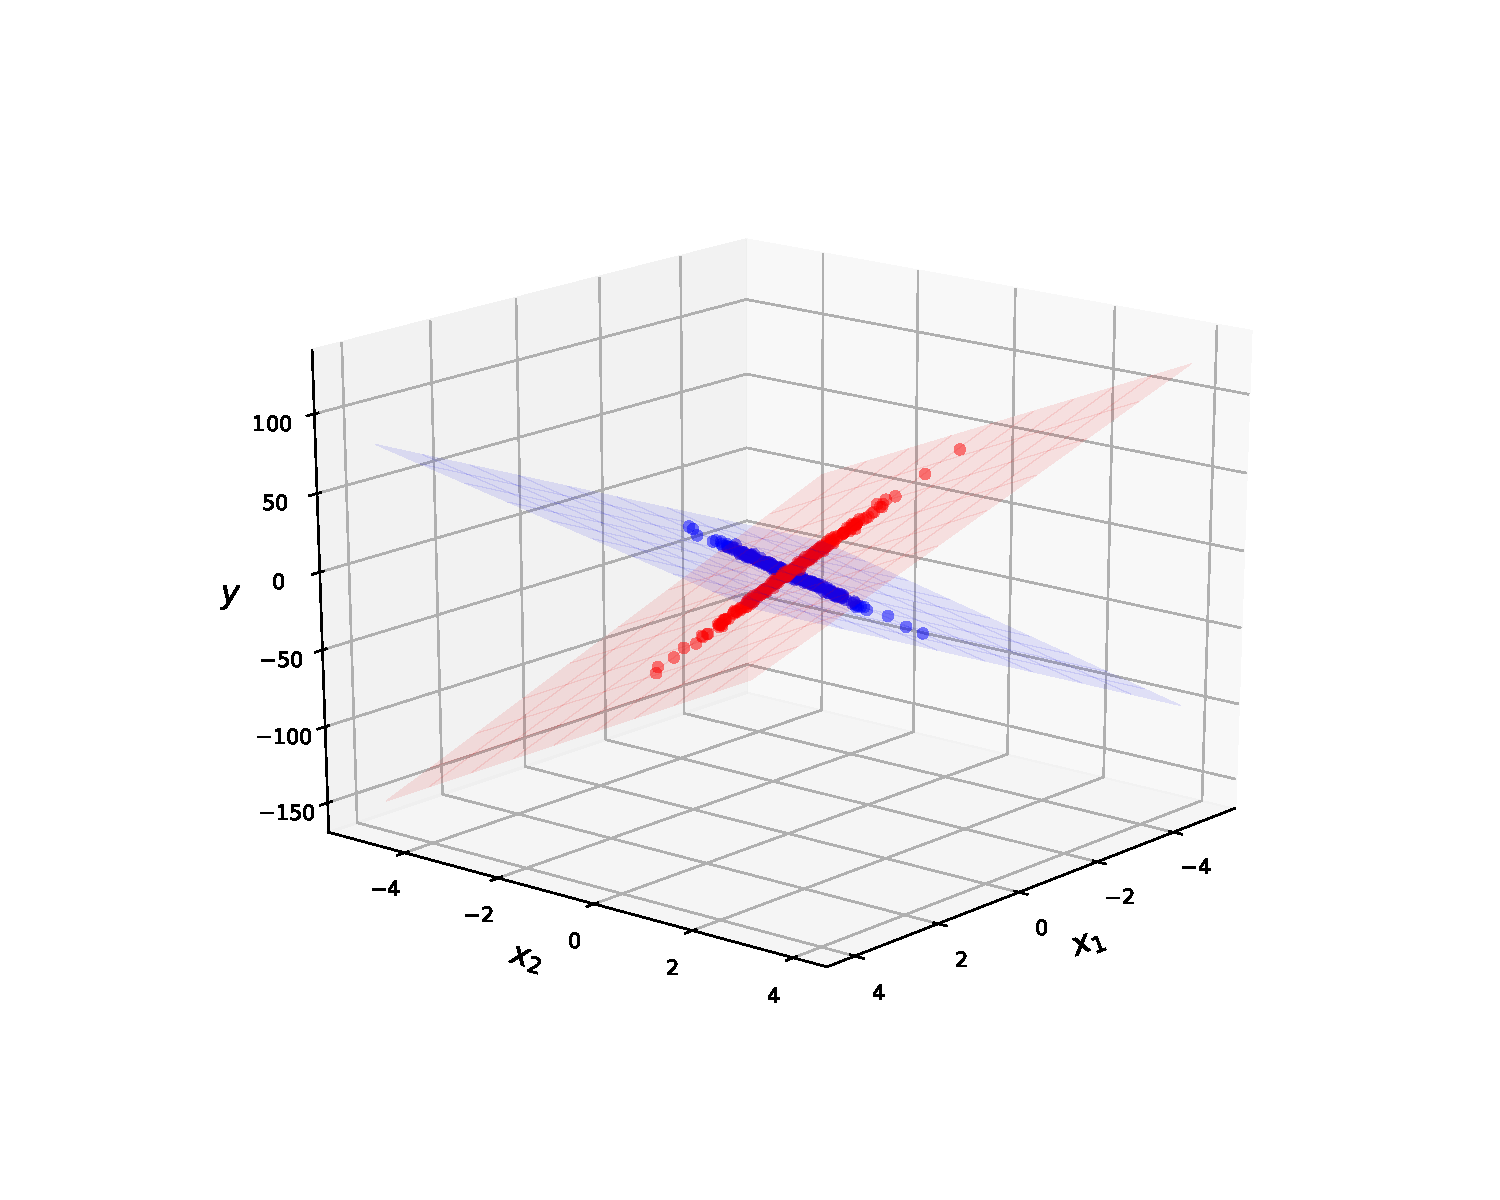
\includegraphics[width=1.2\linewidth]{experiment1-zeros.pdf}  а) \end{center}
\end{minipage}
\hfill
\begin{minipage}[h]{0.49\linewidth}
\begin{center}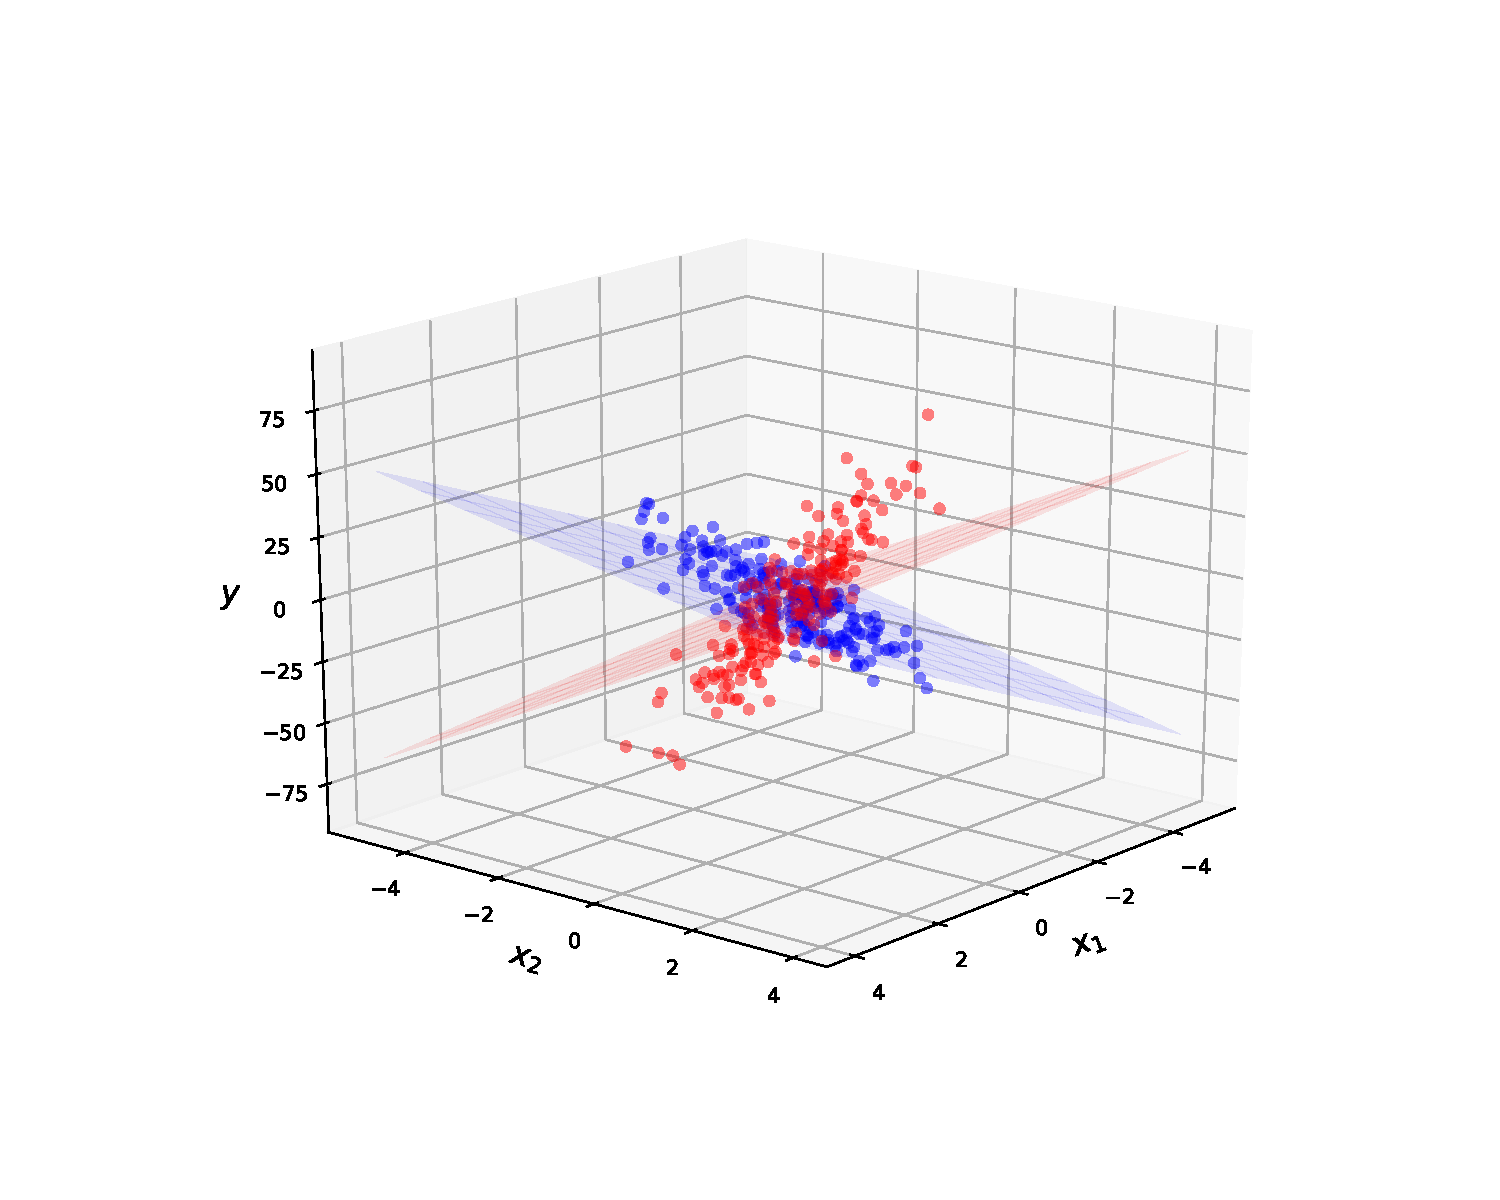
\includegraphics[width=1.2\linewidth]{experiment1-random.pdf}  б) \end{center}
\end{minipage}
\caption{а) Признаки, соответствующие другому подмножеству, заполнялись нулями, б) признаки, соответствующие другому подмножеству, заполнялись случайными числами. Точки соответствуют правильным ответам, плоскости задают предсказание линейной модели для каждого из подмножеств.}
\label{ris:image1}
\end{center}
\end{figure}


Данный эксперимент показывает, что для аппроксимации выборки, порожденной несколькими источниками, одна модель не подходит. Таким образом, при построение модели для обучения нужно учитывать гипотезу порождения данных. Нередко оказывается, что данные порождены несколькими источниками. В этом случае для лучшей аппроксимации можно использовать ансамбль локальных моделей, где каждая локальная модель обрабатывает свою область признакового пространства (в одной области объекты имеют схожие признаки, объекты из разных областей имеют разные признаковые описания).

\subsection{Решение проблемы при помощи ансамбля локальных моделей}

Данный эксперимент ставится для того, чтобы показать, что ансамбль локальных моделей хорошо аппроксимирует выборку, порожденную несколькими источниками.


В данном эксперименте для аппроксимации используется ансамбль двух линейных локальных моделей. 

В первом эксперименте ансамбль обучается на выборке $(\mathbf{y}, \mathbf{X})$, а во втором --- на выборке $(\mathbf{y}, \mathbf{\hat{X}})$. Ансамбль двух линейных локальных моделей хорошо аппроксимирует обе выборки (см. рис. $2$ а, б).  


Данный эксперимент показывает, что ансамбль из двух локальных моделей хорошо аппроксимирует выборку, порожденную несколькими источниками. Качество аппроксимации ансамбля моделей выше, чем при использовании лишь одной модели. 


\newpage
\begin{figure}[h]
\begin{center}
\begin{minipage}[h]{0.49\linewidth}
\begin{center}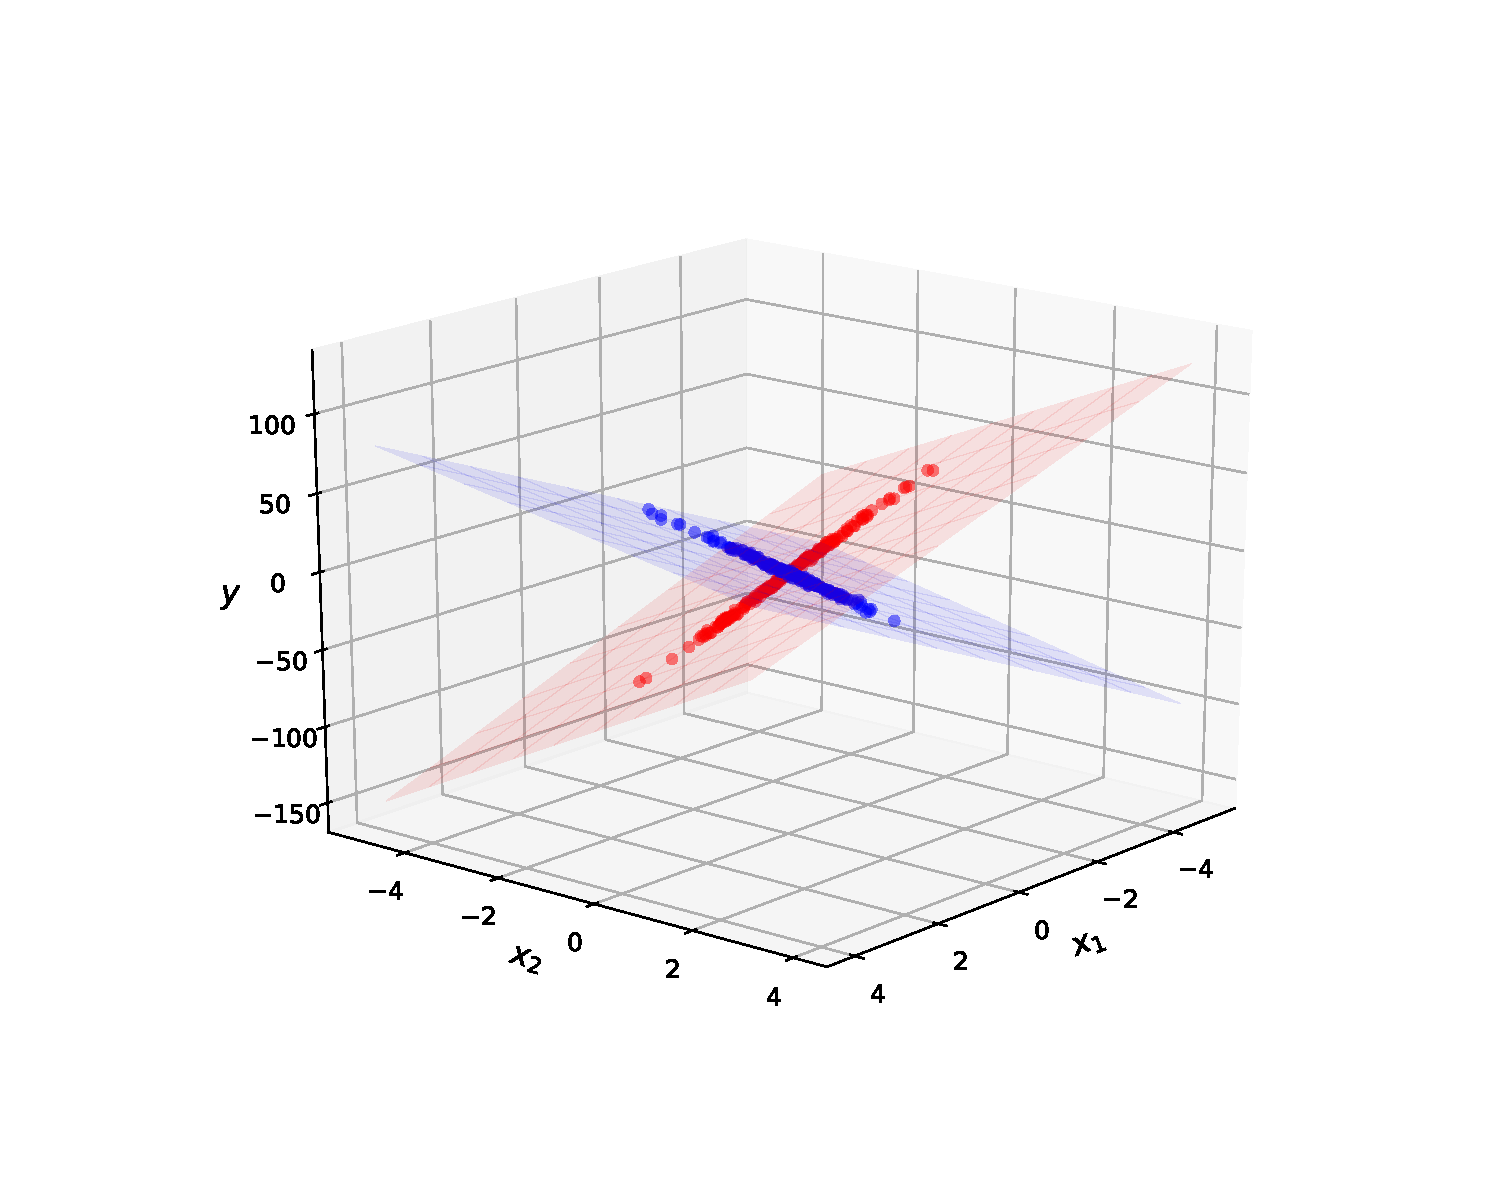
\includegraphics[width=1.2\linewidth]{experiment2-zeros.pdf}  а) \end{center}
\end{minipage}
\hfill
\begin{minipage}[h]{0.49\linewidth}
\begin{center}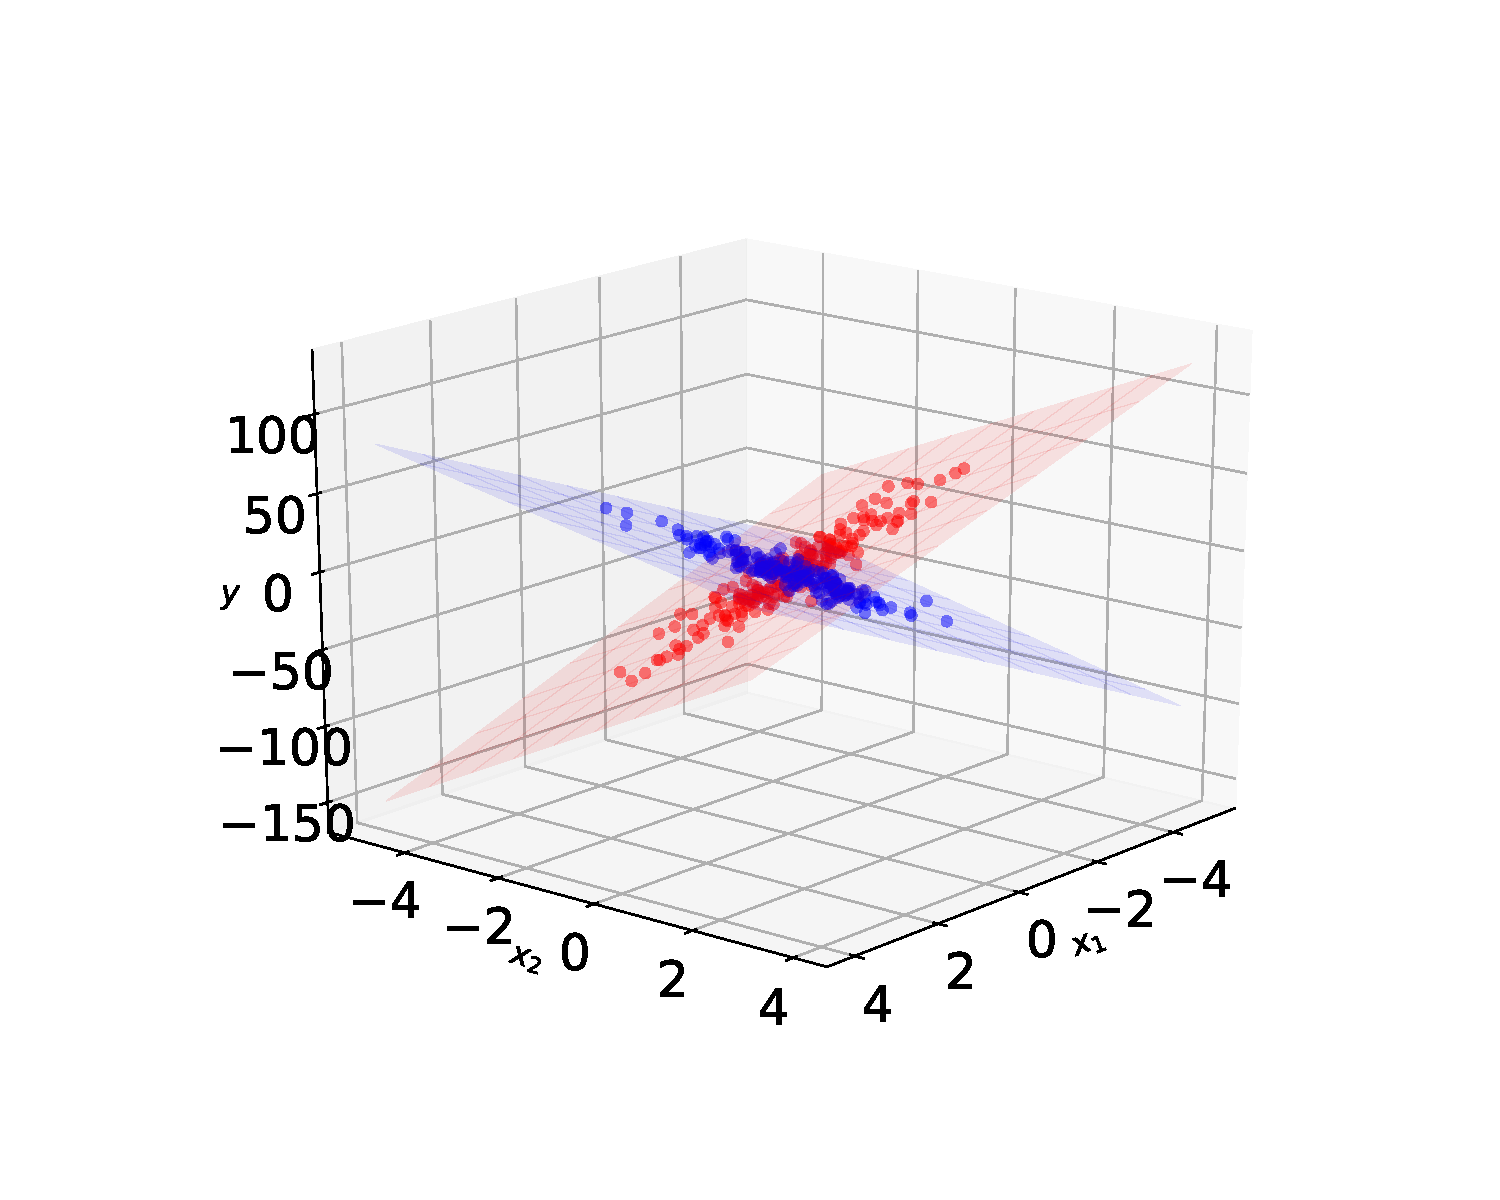
\includegraphics[width=1.2\linewidth]{experiment2-random.pdf}  б) \end{center}
\end{minipage}
\caption{а) Признаки, соответствующие другому подмножеству, заполнялись нулями, б) признаки, соответствующие другому подмножеству, заполнялись случайными числами. Точки соответствуют правильным ответам, плоскости задают предсказание мультимодели для каждого из подмножеств.}
\label{ris:image1}
\end{center}
\end{figure}



\subsection{Анализ ансамбля моделей в зависимости от уровня шума}

\textbf{Синтетические данные.} В качестве данных используются синтетические данные. Используется две подвыборки, каждая из которых описывается линейной моделью с нормальным шумом:
\[\mathrm{y}_m = \alpha_{m}\mathrm{x}_m+ \varepsilon, \qquad x_m, y_m \in \real, \qquad m \in \{1,2\},  \qquad \varepsilon \in \mathcal{N}(0, 1). \eqno(3.4)\] 

В качестве общей выборки рассматривается конкатенация двух подвыборок, описываемая вектором целевой переменной $\mathbf{y}$ и матрицей признаков $\mathbf{\hat{X}}$:	
\[\mathbf{y} = \begin{pmatrix}
\mathrm{y}_1\\
\mathrm{y}_2
\end{pmatrix},\qquad  \mathbf{\hat{X}} = \begin{pmatrix}
\mathrm{x}_1 & \varepsilon_1\\
\varepsilon_2 & \mathrm{x}_2
\end{pmatrix},\eqno(3.5)\]
где $\varepsilon_1, \varepsilon_2 \in \mathcal{N}(0,\sigma)$. На общей выборке обучается ансамбль из двух локальных моделей, каждая из которых является линейной. Исследуется зависимость введенного расстояния $(2.9)$ от параметра шума $\sigma$. График представлен на рисунке $3$.

\begin{figure}[h]
\center{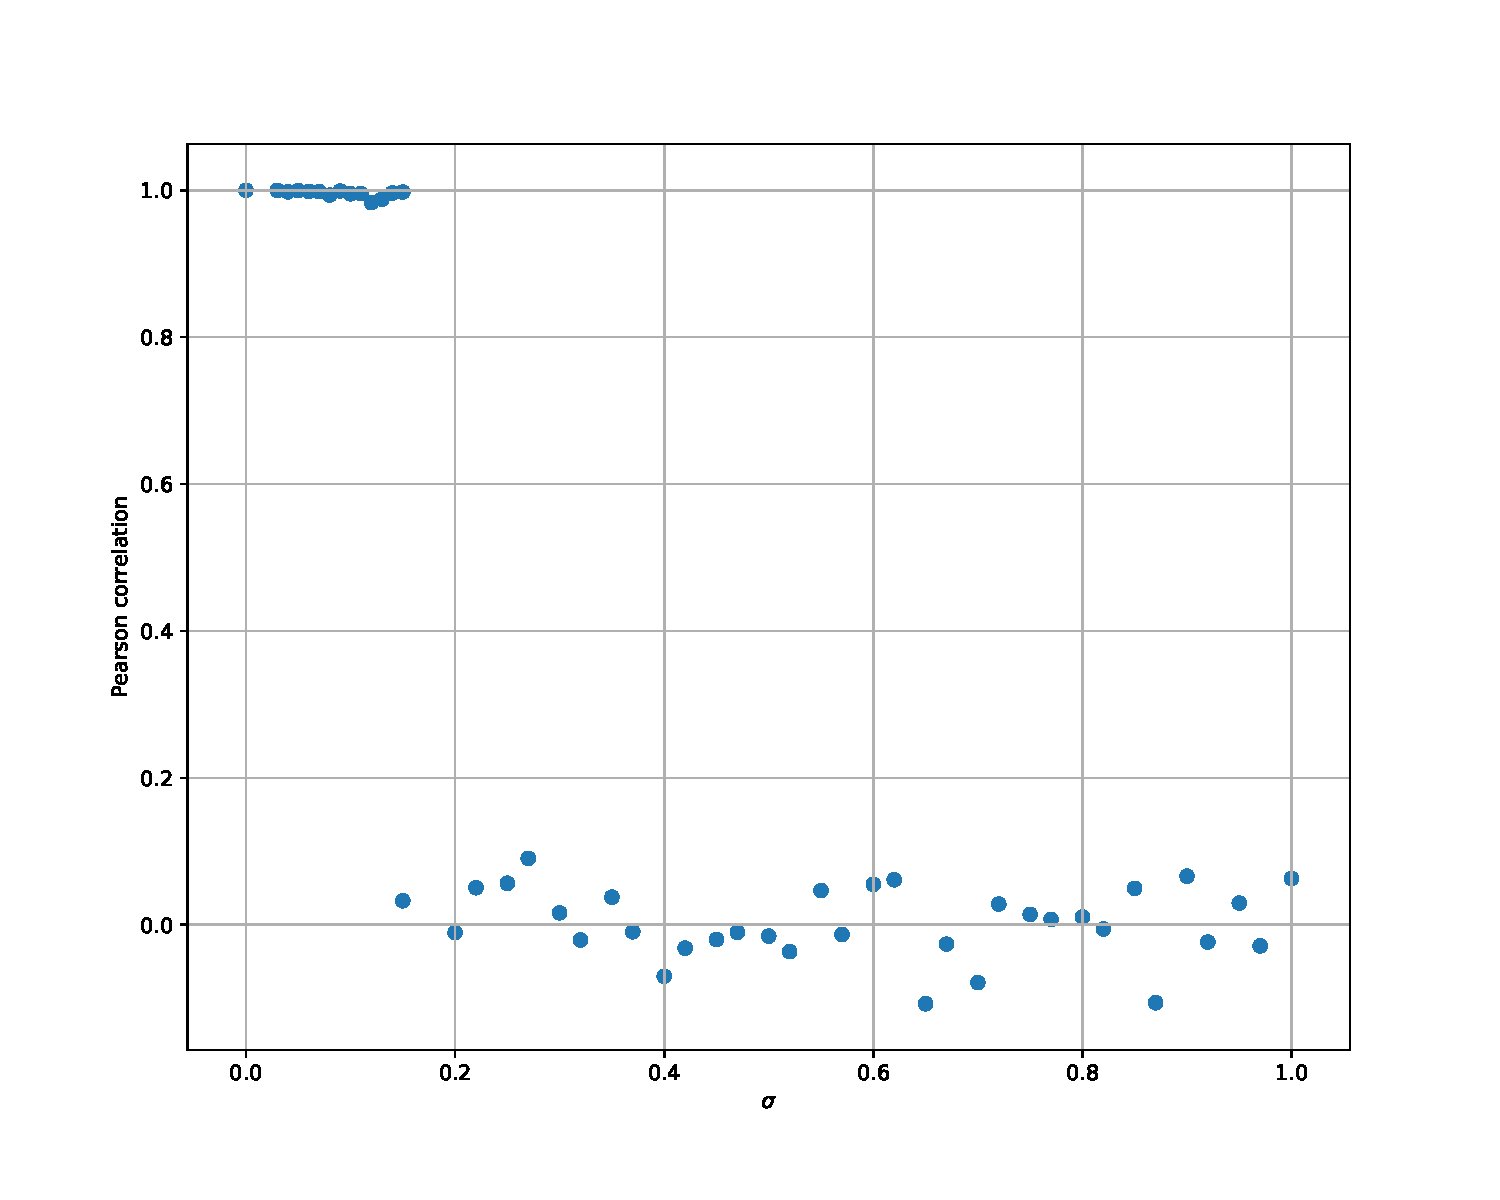
\includegraphics[width=0.7\linewidth]{Pearson_cor_sigma_synthetic.pdf}}
\caption{График зависимости расстояние между локальными моделями от параметра шума $\sigma$ для синтетических данных.}
\label{ris:image}
\end{figure}


На графике видно, что при малом параметре шума $\sigma$ (меньшем, чем пороговое значение) локальные модели близки, корреляция между ними приблизительно равна единице. Это означает, что при малом параметре $\sigma$ шум практически не влияет на данные, для аппроксимации выборки достаточно одной линейной модели, поэтому параметры двух локальных моделей становятся приблизительно одинаковыми. 

На графика также видно, что при параметре шума $\sigma$ большем, чем пороговое значение, локальные модели становятся независимыми друг от друга, корреляция между ними приблизительно равна нулю. Это означает, что шумовые признаки сказываются на данных и для аппроксимации выборки необходимы две модели.

\textbf{Данные на основе выборок Boston housing и Servo.} Выборки Boston housing и Servo описываются матрицами признаков $\mathbf{X}_{b} \in \real^{506\times 13}$ и $\mathbf{X}_s\in \real^{167\times 4}$, а также векторами целевой переменной $\mathbf{y}_b \in \real^{506}$ и $\mathbf{y}_s \in \real^{167}$. В качестве общей выборки рассматривается конкатенация выборок Boston housing и Servo, описываемая вектором целевой переменной $\tilde{\mathbf{y}}$ и $\tilde{\mathbf{X}}$:

\[\tilde{\mathbf{y}} = \begin{pmatrix}
\mathbf{y}_b\\
\mathbf{y}_s
\end{pmatrix} \in \real^{673}, \qquad \tilde{\mathbf{X}} = \begin{pmatrix}
\mathbf{X}_b\\
\mathbf{X}_s ~~\mathbf{\mathcal{E}}
\end{pmatrix} \in \real^{673\times 13},\eqno(3.6)\]
где $\mathbf{\mathcal{E}}$ --- матрица размера $167\times 9$, каждый элемент которой из $\mathcal{N}(0,\sigma)$. На общей выборке обучается ансамбль из двух локальных моделей, каждая из которой является линейной. Исследуется зависимость расстояния между локальными моделями от параметра шума $\sigma$. График представлен на рисунке $4$:


\begin{figure}[h]
\center{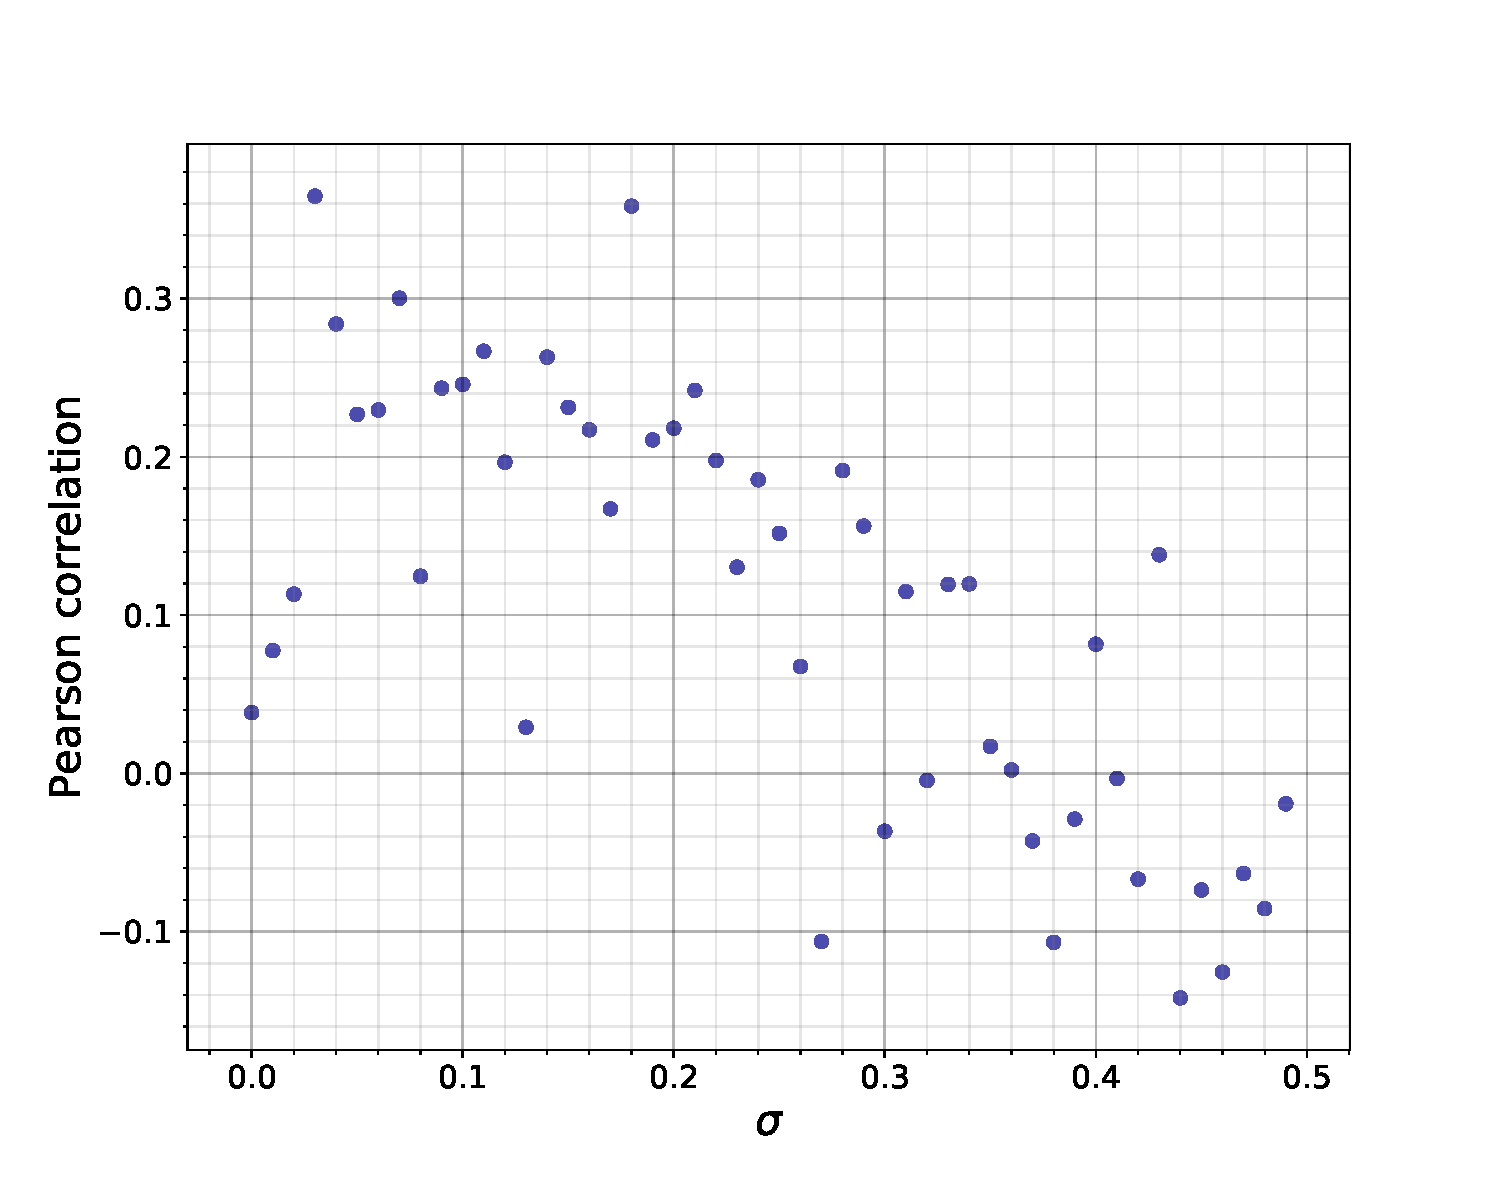
\includegraphics[width=0.7\linewidth]{Pearson_cor_sigma_boston_and_servo.pdf}}
\caption{График зависимости расстояние между локальными моделями от параметра шума $\sigma$ для выборок Boston housing и Servo.}
\label{ris:image}
\end{figure}

На графике видно, что при увеличении параметра шума $\sigma$ есть тенденция к уменьшению скалярного произведения между моделями. Это означает,  с увеличением шума локальные модели отдаляются друг от друга.

Исследуем качество аппроксимации при использовании ансамбля двух линейных локальных моделей. Ошибка аппроксимации вычисляется по формуле

\[\text{error} = \sum_{k=1}^2\sum_{i=1}^N \pi_k(\mathbf{x}_i, \mathbf{w}^k)(\mathrm{y}^{pred_k}_i - \mathrm{y}^{real}_i)^2,\eqno(3.7)\]
где $N = 673$ --- количество объектов в общей выборке, $y_i^{pred_k}$ --- предсказанное значение для $i$-го объекта $k$-ой моделью, а $y^{real}_i$ --- значение целевой переменной $i$-го объекта.  График зависимости ошибки аппроксимации от параметра шума представлен на рисунке $5$:

\begin{figure}[H]
\center{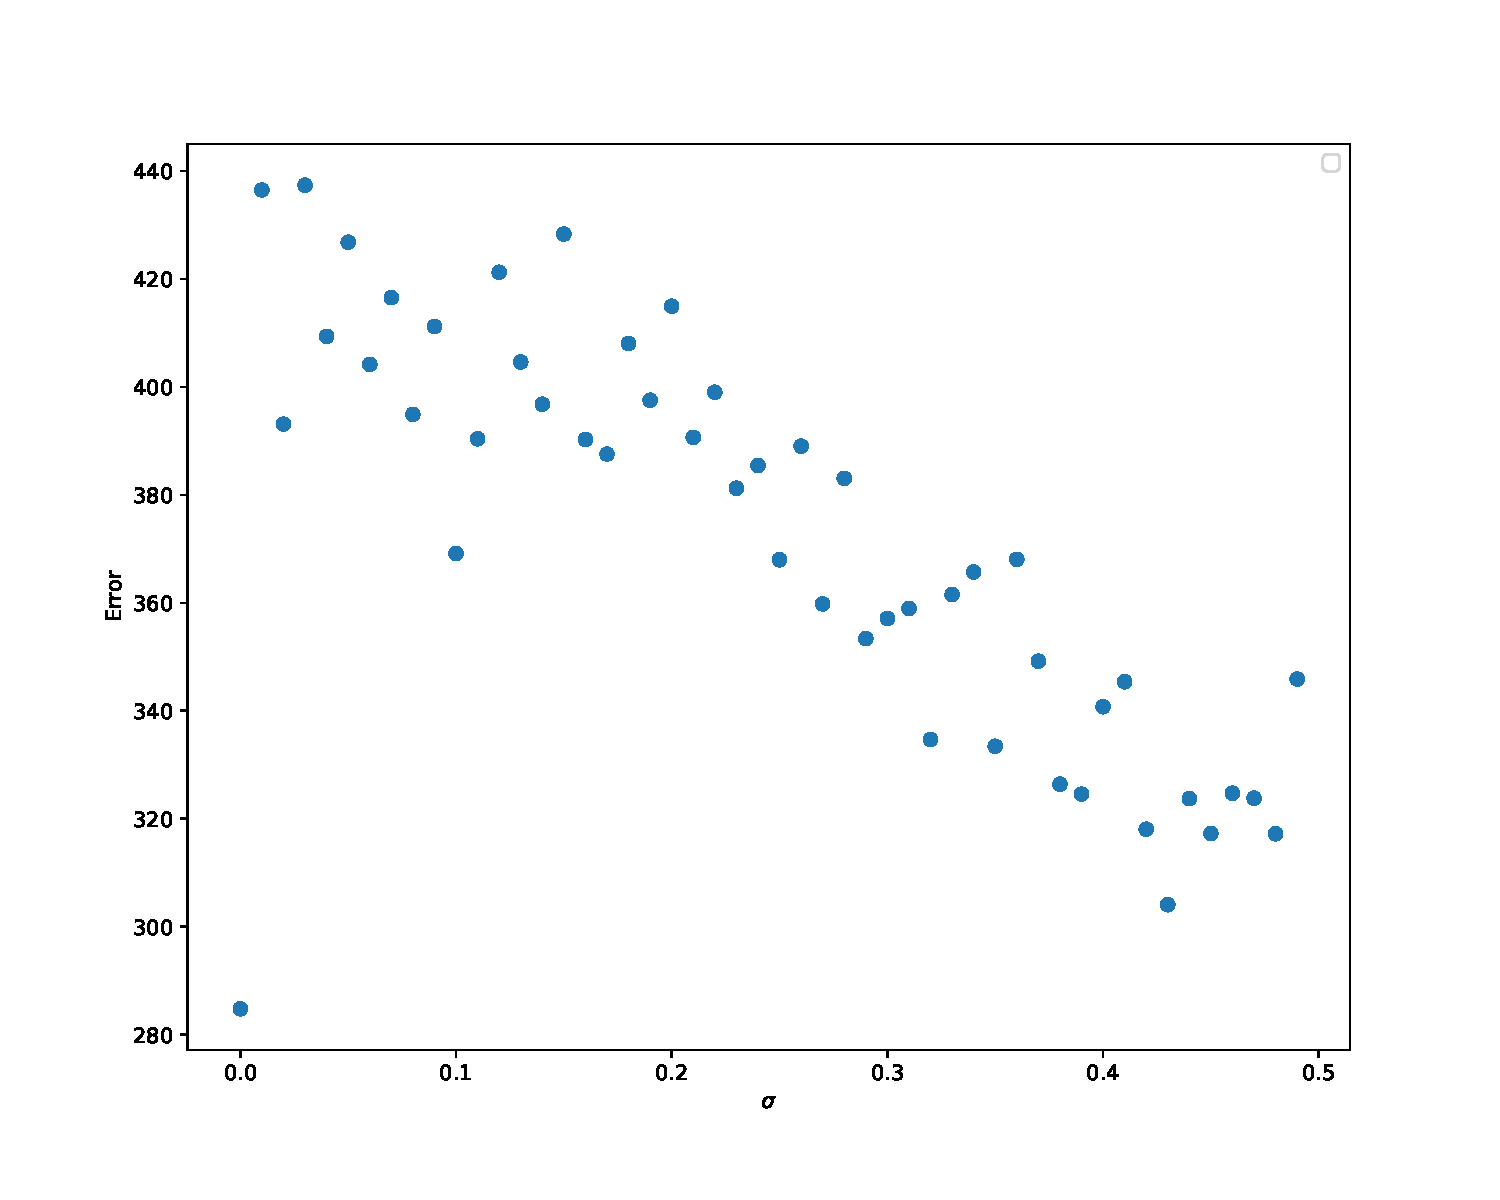
\includegraphics[width=0.7\linewidth]{Errors_sigma_boston_and_servo.pdf}}
\caption{График зависимости ошибки аппроксимации от параметра шума $\sigma$ для выборок Boston housing и Servo.}
\label{ris:image}
\end{figure}

На графике видно, что с ростом параметра шума $\sigma$ ошибка падает, тем самым качество аппроксимации при использовании ансамбля двух локальных моделей увеличивается. Однако ошибки локальных моделей отдельно не уменьшается:


\begin{figure}[h]
\begin{center}
\begin{minipage}[h]{0.49\linewidth}
\begin{center}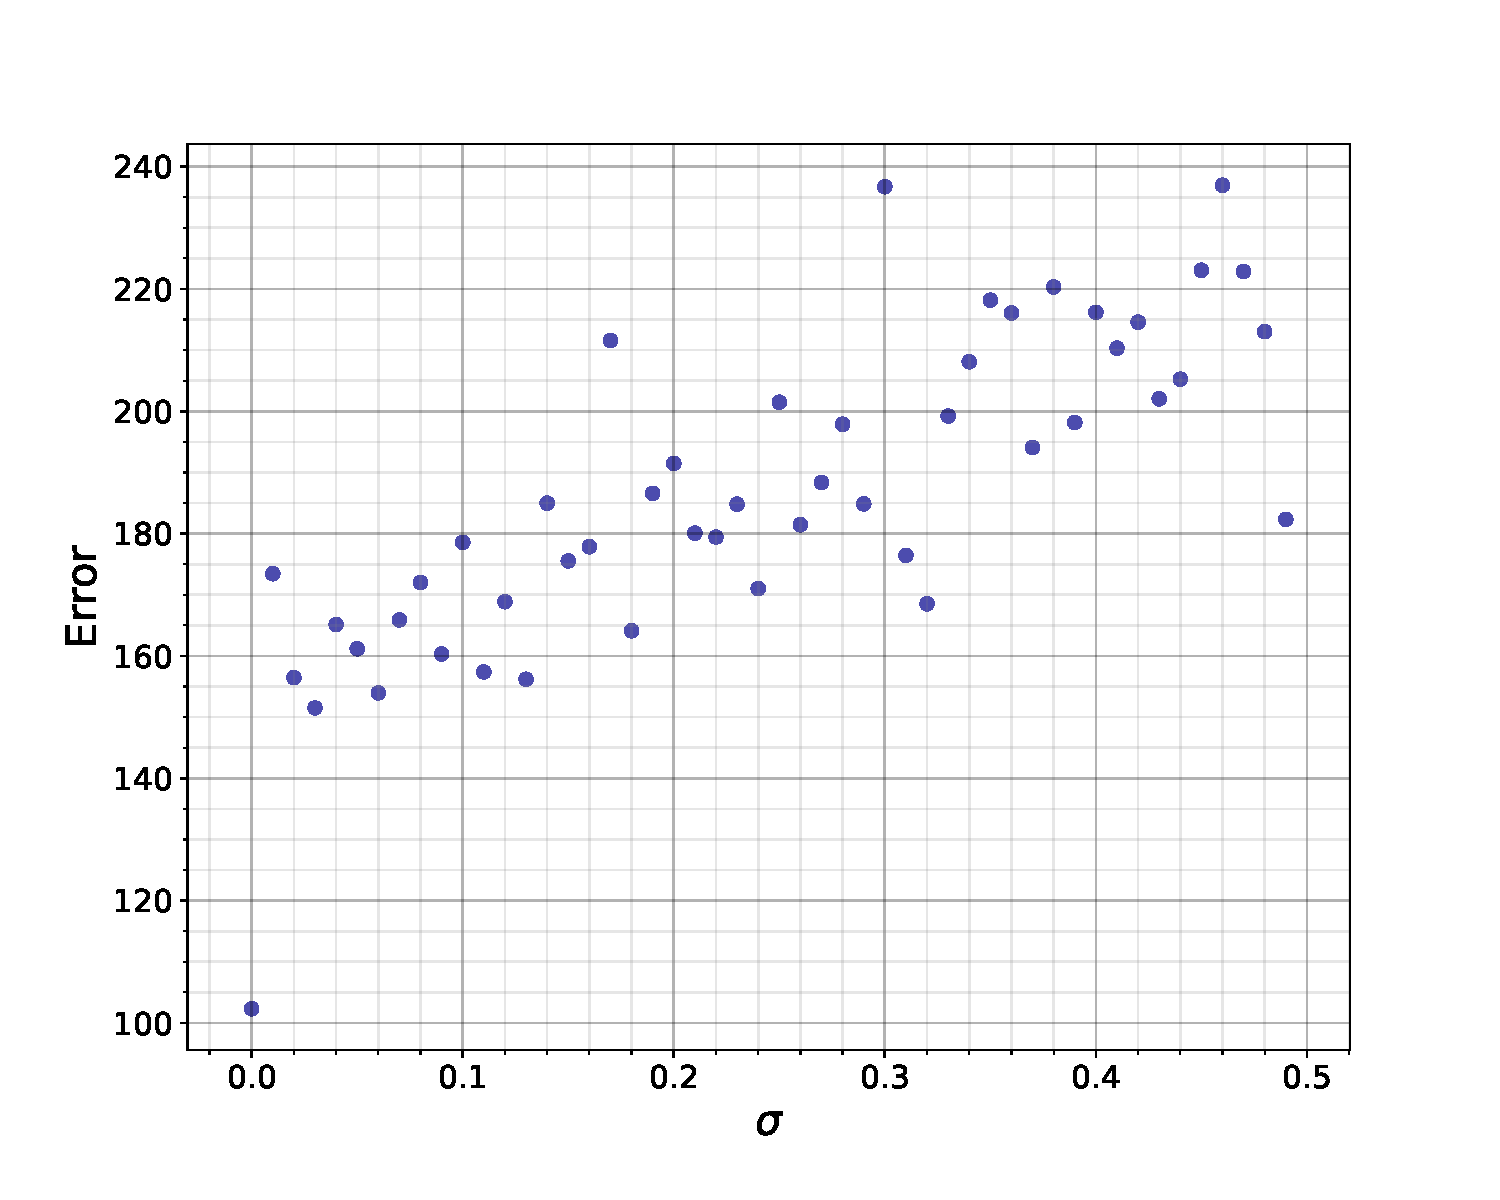
\includegraphics[width=1.1\linewidth]{Errors_sigma_boston_and_servo_model1.pdf}  а) \end{center}
\end{minipage}
\hfill
\begin{minipage}[h]{0.49\linewidth}
\begin{center}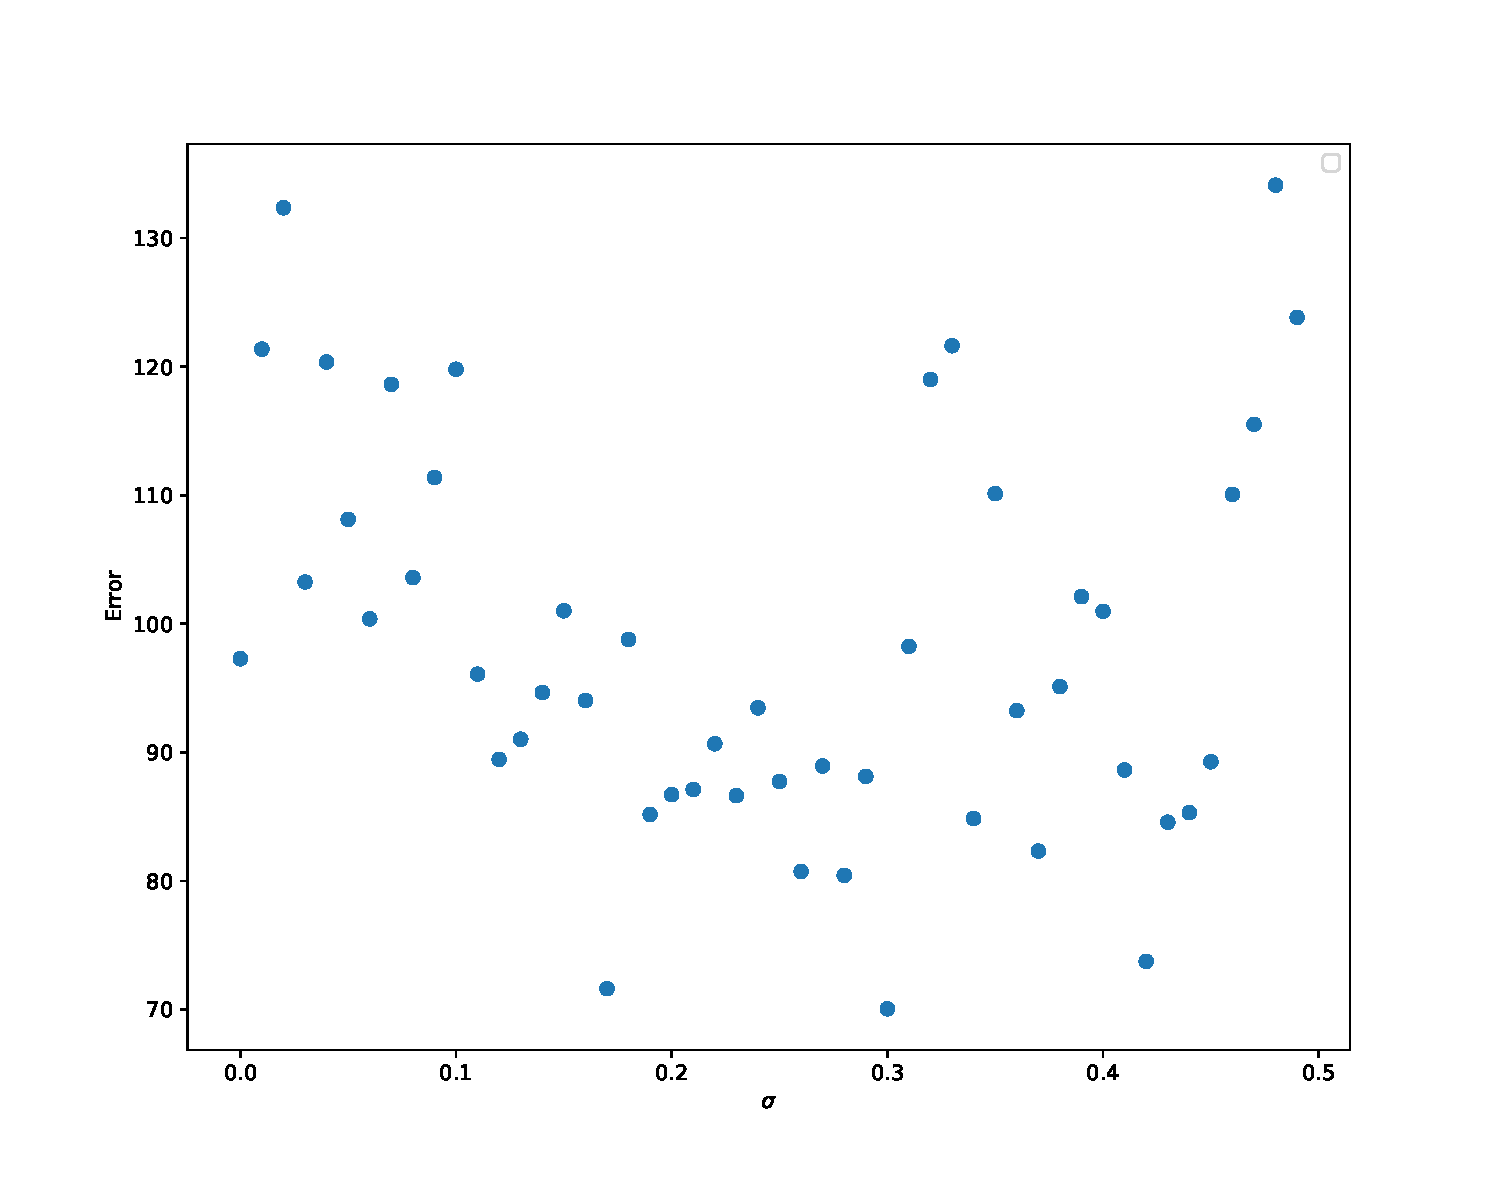
\includegraphics[width=1.1\linewidth]{Errors_sigma_boston_and_servo_model2.pdf}  б) \end{center}
\end{minipage}
\caption{а) График зависимости ошибки аппроксимации от параметра шума $\sigma$ для выборок Boston housing и Servo для а) первой модели ансамбля; б) второй модели ансамбля .}
\label{ris:image1}
\end{center}
\end{figure}

Код для повторения эксперимента можно найти по ссылке на репозиторий \href{https://github.com/Intelligent-Systems-Phystech/2020_Project-51}{github}, в котором расположены все материалы работы.
\section{Заключение}

В данной работе был исследован ансамбль локальных моделей на различных данных, порожденных несколькими источниками. В качестве данных использовались синтетические выборки, а также датасэты Boston housing и Servo. В данной работе в качестве локальной модели использовалась линейная модель, в качестве шлюзовой функции использовалась двухслойная нейросеть. 

Как показано в эксперименте, в случае, когда синтетические данные порождены двумя источниками, ансамбль локальных моделей является более точной, так как лучше аппроксимирует плоскости точек для каждого из источников. 

Также был проведен эксперимент по исследованию качества аппроксимации при использовании ансамбля локальных моделей. Было введено расстояние между локальными моделями, чтобы исследовать поведение локальных моделей между собой. В эксперименте показано, что с ростом параметра шума ошибка аппроксимации отдельной локальной модели не уменьшается, однако ошибка всего ансамбля локальных моделей падает. При этом модели становятся более независимыми, так как расстояние между стремится к нулю при увеличении параметра шума. 

В дальнейшем планируется исследовать оптимальное количество локальных моделей в ансамбле. Планируется использовать функцию расстояния в качестве регуляризатора, чтобы улучшить качество аппроксимации и сделать локальные модели в ансамбле более независимыми.

\bibliographystyle{unsrt}
\bibliography{Islamov}

\end{document}
